%!TEX program = xelatex

% 通过调整aspectratio参数调整屏幕比例 
% 比如4:3就设置aspectratio=43
% 16:9就设置aspectratio=169
\documentclass[aspectratio=169]{mybeamer}
% \documentclass[aspectratio=169,noSy]{mybeamer} 		% 使用思源字体

% 插入中国人民大学统计学院的LOGO
\logo{
\includegraphics[height = 18pt]{RUCstat_logo.png}\hspace{.3cm}\vspace{0.82\paperheight}
}

\title{RUCStatBeamer模板}
\subtitle{制作一个自己的Slides}
\author{Gu}
\date[Aug. 27,2021]{August 27,2021}

\begin{document}
	\frame{\titlepage}
	% \addPartPage 在每一个Part开始前增加转场页
	\addPartPage

	\part{我也不知道是什么}
	% \setToc{} 增加一个目录页,标题为{}内参数
	\setToc{目录}

	% \addSectionPage 在每一个Section前增加导航页
	\addSectionPage

	\section{公式及图片}
	\begin{frame}
		\frametitle{插入公式}
		插入一个带编号的公式
		\begin{equation}
			f(x;\mu,\sigma^2) = \frac{1}{\sqrt{2 \pi} \sigma } e^{-\frac{(x - \mu)^2}{2 \sigma^2}}
		\end{equation}
		也可以插入不带编号的公式
		\begin{equation*}
			\mathbb{P}\{ X = k\} = \frac{\lambda^k}{k!} e^{-\lambda} 
		\end{equation*}
		插入行内公式就比较简单$a^2 + b^2 = c^2$
	\end{frame}

	\begin{frame}
		\frametitle{插入图片}
		\begin{minipage}[c]{.5\textwidth}
			\begin{figure}[htb]
				\centering
				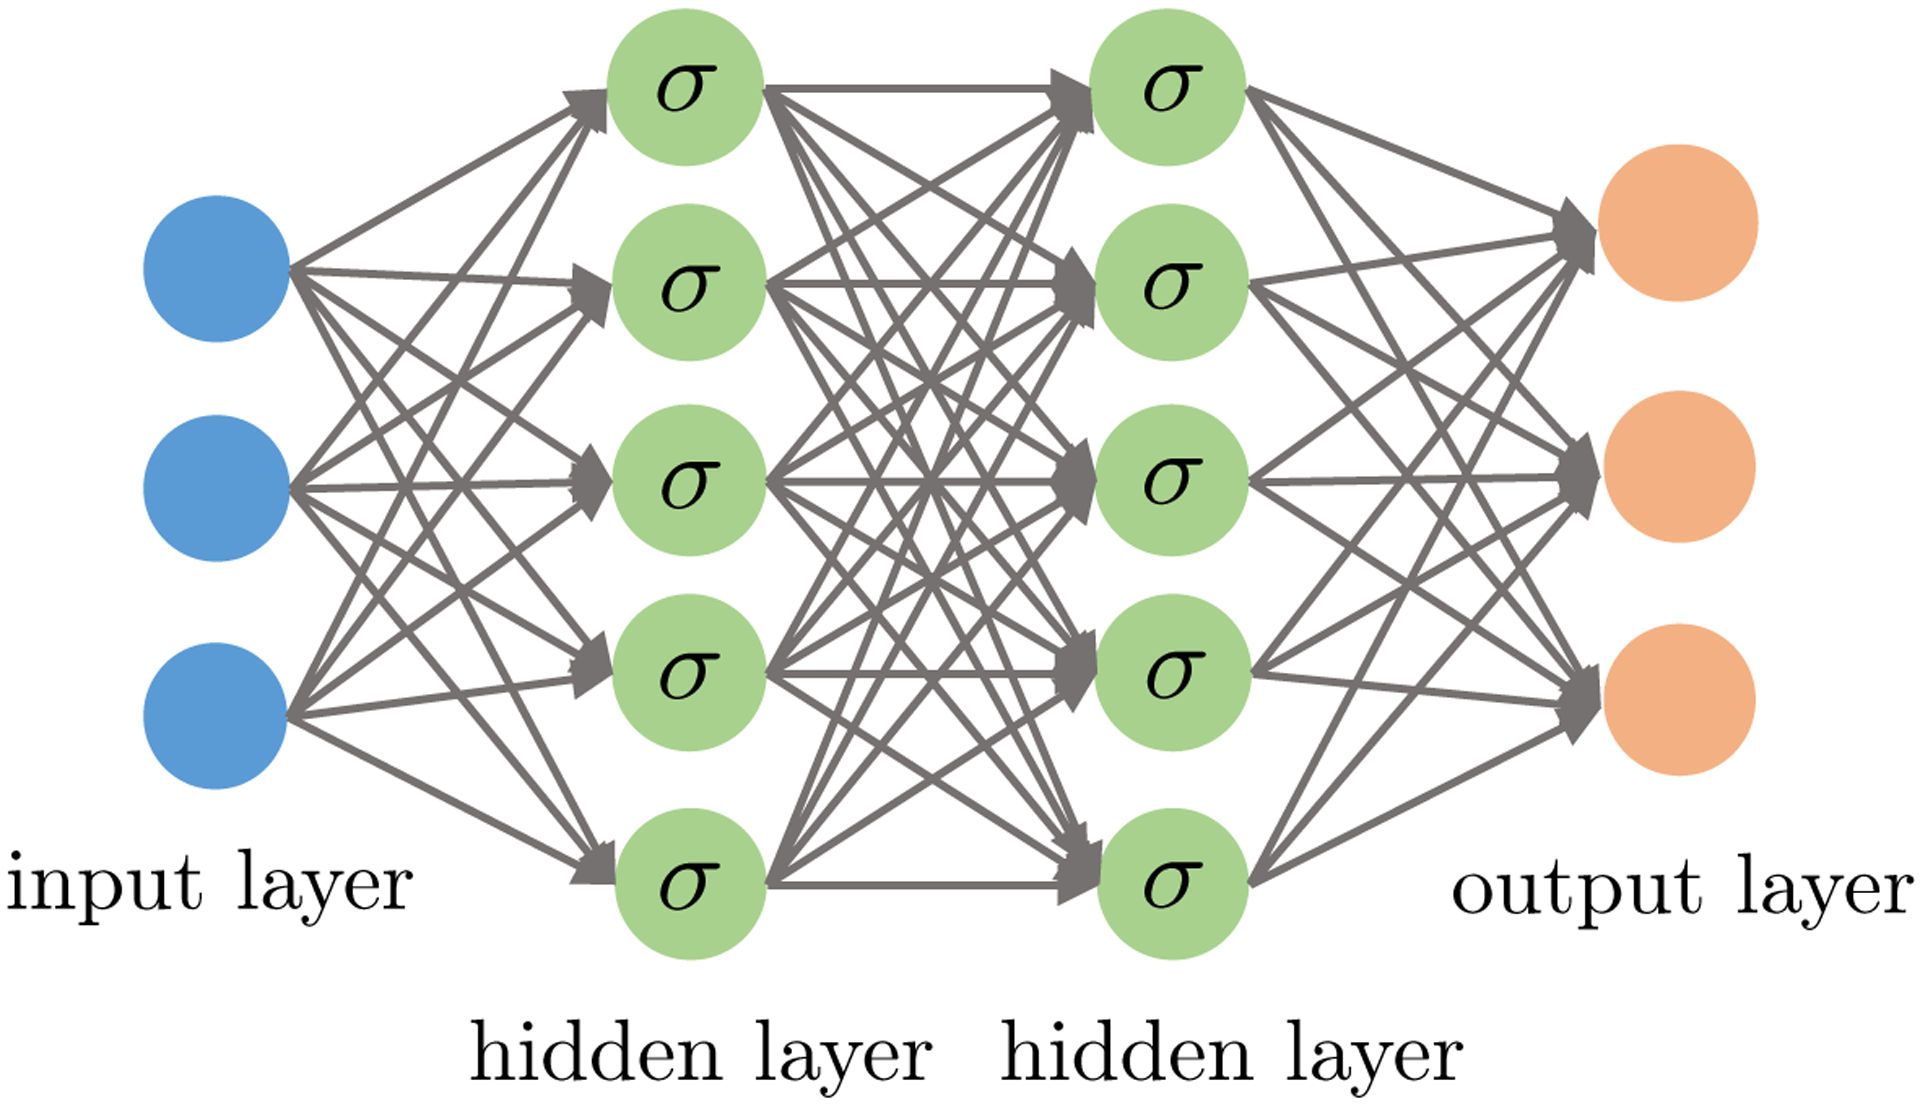
\includegraphics[width=\textwidth]{figures/nn.jpg}
				\caption{神经网络}
			\end{figure}
		\end{minipage}
		\hspace{0.1cm}
		\begin{minipage}[c]{.45\textwidth}
			\begin{itemize}
				\setlength{\itemsep}{1cm}
				\item 前馈网络对于机器学习的从业者是极其重要的。它们是许多重要商业应用的基
				础。
				\item 例如,用于对照片中的对象进行识别的卷积神经网络就是一种专门的前馈网络。
			\end{itemize}
		\end{minipage}
	\end{frame}

	\section{列表环境}
	\begin{frame}
		\frametitle{无序列表和有序列表}
		可以插入有序列表
		\begin{enumerate}
			\item 第一,绝对不意气用事
			\item 第二,绝对不漏抓任何一件坏事
			\item 第三,绝对裁判得公正漂亮
		\end{enumerate}
		同样也可以插入无序的列表
		\begin{itemize}
			\item 通过无序的列表表达并列关系
			\item 列表也可以进行嵌套
			\begin{itemize}
				\item 看,这是1层嵌套
			\end{itemize}
		\end{itemize}
	\end{frame}

	\section{块环境}
	\begin{frame}
		\frametitle{插入一般的块}
		\begin{block}{贝叶斯规则}
			我们经常会需要在已知$P(y|x)$时计算$P(x|y)$。幸运的是,如果还知道$P(x)$,
			我们可以用\textbf{贝叶斯规则}(Bayes' rule)来实现这一目的:
			$$
			P(x|y) = \frac{P(y|x) P(x)}{P(y)}
			$$
		\end{block}
	\end{frame}
	\begin{frame}
		\frametitle{插入定理环境}
		\begin{theorem}[Stokes定理]
			$$
			\int_{\partial \Omega} \omega = \int_{\Omega} \mathrm{d} \omega	
			$$
		\end{theorem}
	\end{frame}
\end{document}
